% chap5.tex (Definitions, Theorem and Proof)

%\chapter{CPS Device Sensor Data Anomaly Detection using Provenance Graphs}
%\chapter{Anomaly Detection using Provenance Graphs}
\chapter{Provenance-Based Anomaly Detection} \label{sec:prov_anomaly}
This chapter discusses the application of provenance data for intrusion detection of malicious events in a CPS device. We propose an approach to identifying anomalous sensor events using provenance graphs. This approach involves the use of a similarity metric to compare observed provenance graphs with provenance graphs derived from an application's normal execution. The result is an anomaly score which is  compared with a previously set threshold to classify an observed provenance graph as either anomalous or benign. We evaluate the effectiveness of our approach with a sample IoT application that simulates a climate control system.
 
 \par Our method of comparing the similarity of provenance graphs was inspired by an information retrieval technique for document retrieval. Given a corpus $D = \{ d_1,..., d_n\}$, and query, $q$, how do we find document(s) $\{d_x,....d_y\}$ which are similar to $q$ and rank them by order of importance. To achieve this, documents contained in the corpus are converted into a vector space representation which allows documents to be ranked based on some similarity metric.


\section{Graph Similarity} \label{similarity}
Similarity is a measure of how identical two objects are, for example, by measuring the angle between objects (using cosine similarity) or a linear distance (using euclidean distance) between the objects. In this work, we use cosine similarity, a widely used similarity metric in information retrieval that has been shown to perform well with sparse datasets. Cosine similarity is a measure of orientation between two non-zero vectors. It measures the cosine of the angle between the vectors. Two vectors which are at an angle of 90$\degree$ have a similarity of 0, two vectors which are identical (with an angle of 0\degree) have a cosine of 1, and two vectors which are completely opposite (with an angle of 180\degree) have a similarity of -1. Since we are concerned with the similarity between vectors, we are only concerned with the positive values bounded in [0,1]. The cosine similarity between two vectors, $X$ and $Y$, is computed by:

\[\mathbf{\cos{(\theta)}} = \dfrac{X \cdot  Y}{ \lVert \mathbf{X} \rVert \cdot \lVert \mathbf{Y} \rVert} =\dfrac{\sum_{i}^n X_i Y_i }{\sqrt[]{\sum_{i}^n X_i^2} \times \sqrt[]{\sum_{i}^n Y_i^2}}  \]

%Algorithm \ref{alg:graph_similarity} describes how to calculate the cosine similarity of two graphs $p_x, p_y$ given their vector representations $u_x, u_y$

%Each graph consist of an edge list which contains all edges contained in the provenance graph.

\par In order to apply cosine similarity between provenance graphs, we compute a vector representation which reduces the graph into an $n$-dimensional vector space where $n$ represents the total number of edges contained in the union of all edge sets. Figure \ref{prov_vector} illustrates the vector space conversion of provenance graphs. $\boldsymbol{G_1}$, and $\boldsymbol{G_2}$ which consists of vertices $A,B,E,F,G, I, J, L, S, R$ and edge labels $used, wAW, wGB, wDB$. The vector space representation of $u_1$ is the occurrence of edges contained in the edge set of graph $G_1$, which  are also found in the collective union of edge sets. Algorithm \ref{graph_to_vector} further outlines the concept of graph to vector conversion.

\begin{figure}[h!]
\begin{center}
%\includegraphics[width=\textwidth]{vector3.pdf}
%\includegraphics[width=\textwidth]{vector5.pdf}
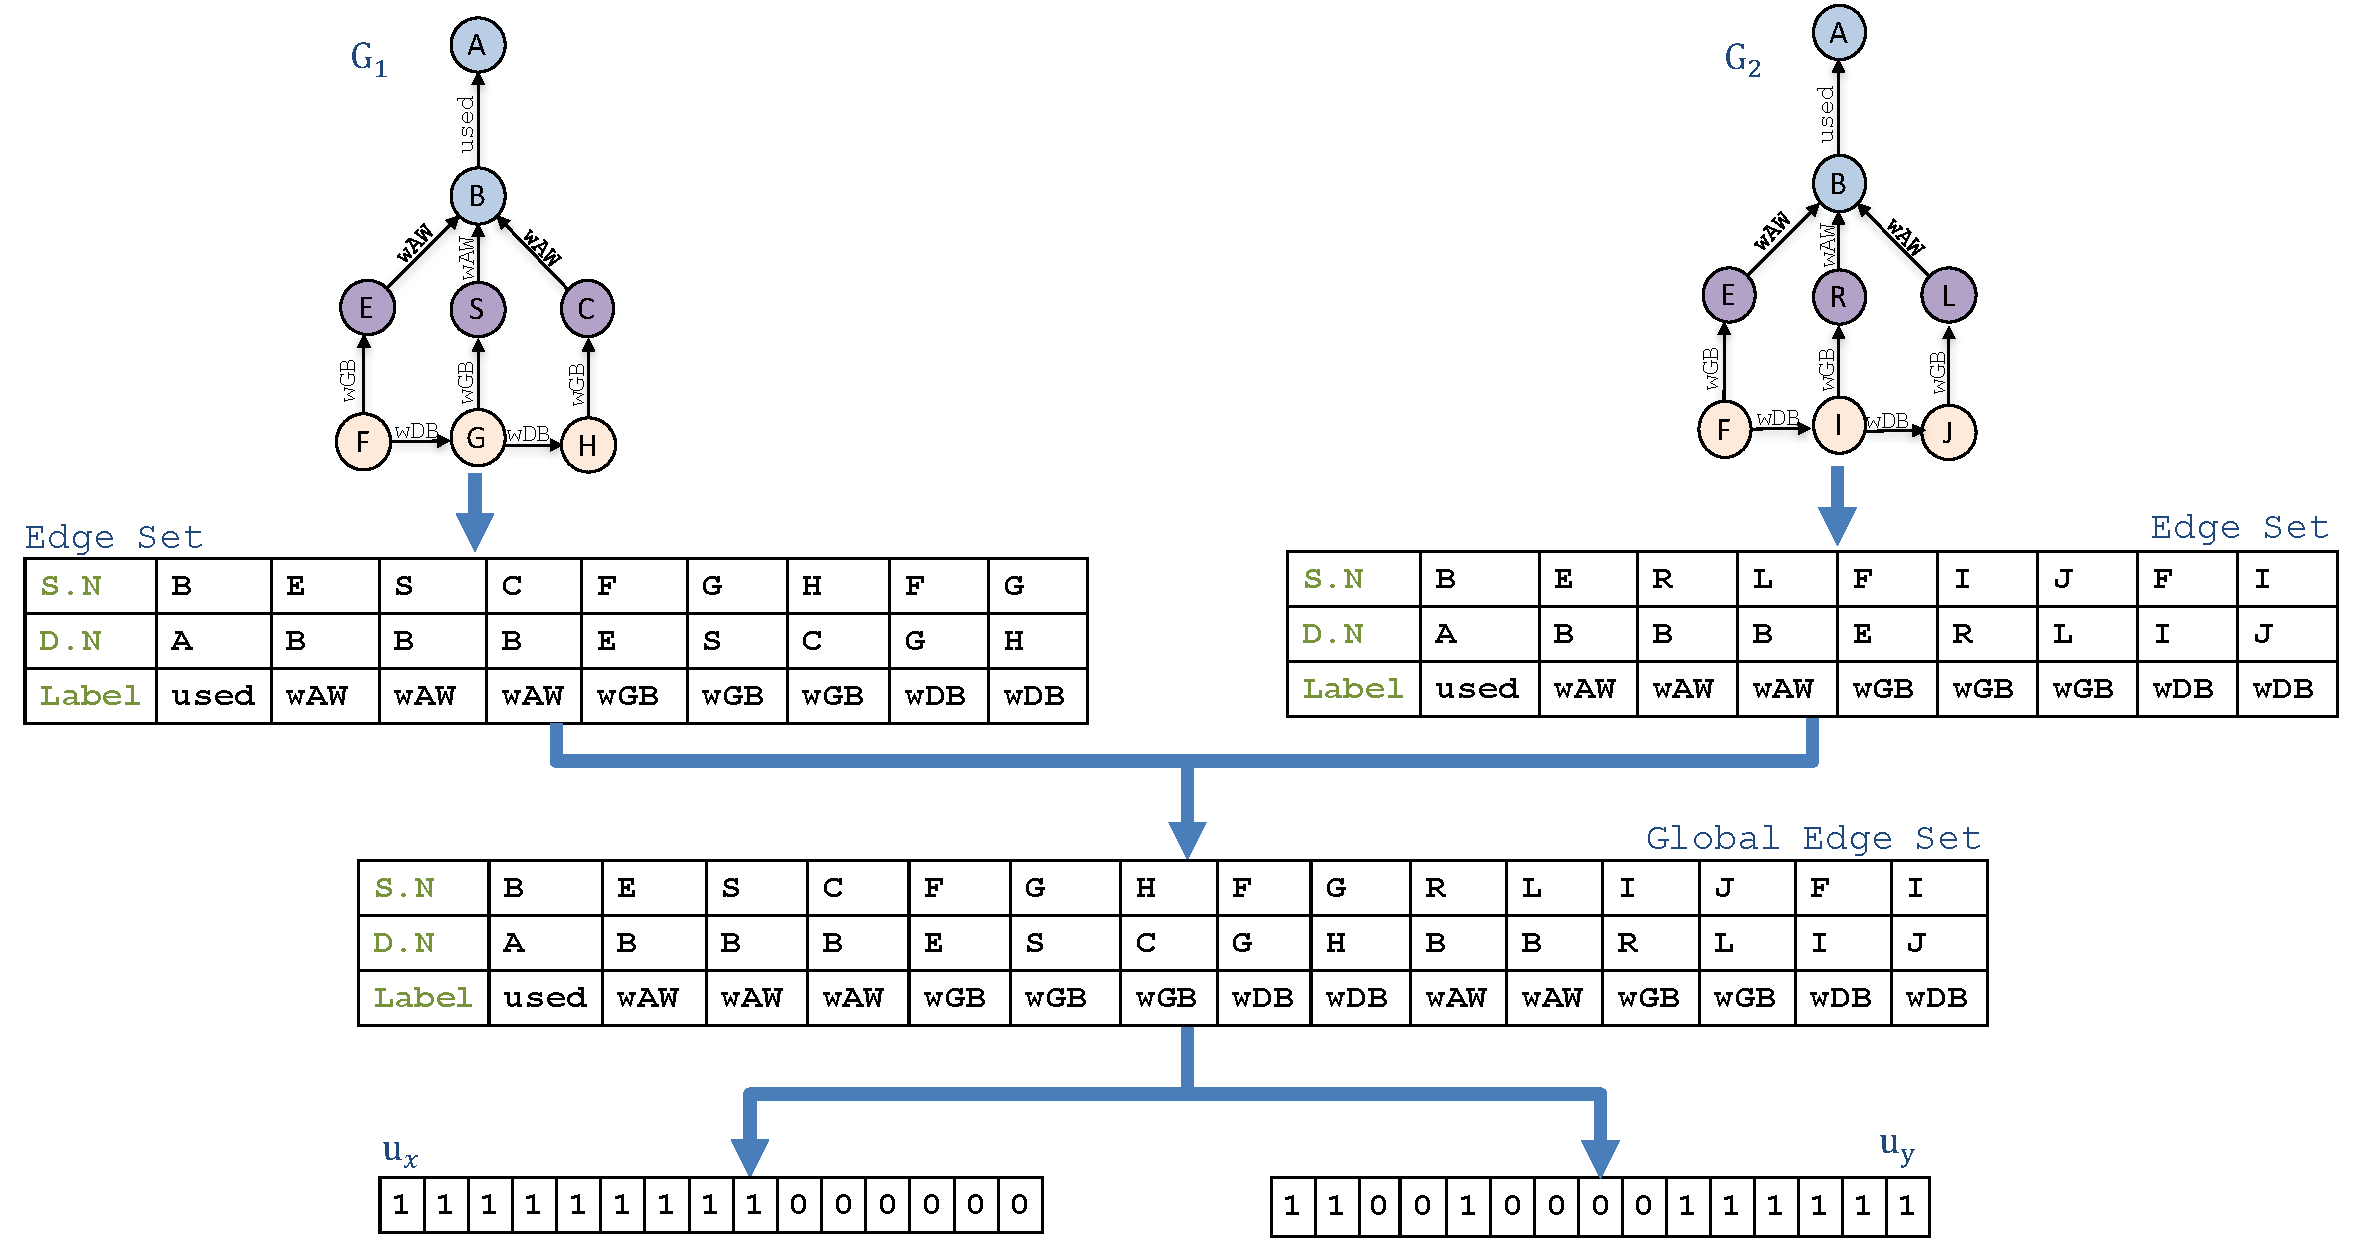
\includegraphics[width=\textwidth]{Picture_13_edit_5.pdf}
\end{center}
\caption{Provenance graph conversion to vector space. $u_x, u_y$ represents vectors generated from both provenance graphs and labels are an abstraction of $(type, value)$ tuple. }
\label{prov_vector}
\end{figure}

\section{Anomaly Detection on Provenance Graphs}
Anomaly detection involves the use of rule-based, statistical, clustering or classification techniques to determine normal or anomalous data instances. The process of determining all anomalous instances in a given dataset is a complex task. A major challenge in anomaly detection is providing the right feature set from the data to use for detection. Another challenge exists in defining what constitutes as normal system behavior. Most anomaly detection using point-based data often fail to include the dependencies that exist between data points. 

\begin{algorithm}[h!]  
\caption{Graph to vector conversion.} 
 \label{graph_to_vector} 
\begin{algorithmic}[1]

\Procedure{GraphtoVector}{$E, E_G$}

\State $n \gets |E_G|$

\State $Q[k],Q[i] \gets 0, 0 \leq i < n$

\For{$e_j \in E$}

%\State \textit{Found} $\gets$ \textbf{False}

\For{$e_g \in E_G \mid 0 \leq g < n$}

%\If{$e_j \sim e_g$}
\If{$e_j = e_g$}
\State $Q[g] \gets Q[g] + 1$
%\State \textit{Found} $\gets$ \textbf{True}
\EndIf

\EndFor

\EndFor


\State \textbf{return} $Q$

\EndProcedure

\end{algorithmic}
\end{algorithm}


\begin{algorithm}[h!]

\caption{Detection algorithm given an observation phase graph set, $P$, a detection phase graph, $G$, and a threshold $T$.} 
 \label{alg:graph_anomaly} 

\begin{algorithmic}[1]  

\Procedure{GraphAnomaly}{$P,G,T$}

\State \textbf{INPUT: } $P=\{G_0,...,G_n\} \mid G_i\gets (V_i, E_i), 0 \leq i \leq n.$

%\State $E_G \gets \{\}$
%\For{$p_i = (V_i, E_i) \in P, 0 \leq i \leq n$}
\State $E_G \gets \cup_{i=0}^{n} E_i$

\State $G \gets (V, E)$

\State $Q \gets GraphtoVector(E, E_G)$ 

\State $Z \gets \{\}$

\For{$G_i \in P$}
\State $N_i \gets GraphtoVector(E_i, E_G)$

\State $z \gets Cosine\_Similarity(Q, N_i)$

\State $Z \gets Z \cup z_i$

\EndFor	

\State $s_{val} \gets max(Z)$

\If{ $s_{val} \geq T$}
\State \textbf{return} normal

\EndIf

\State \textbf{return} anomaly
\EndProcedure
\end{algorithmic}
\end{algorithm}

\par Many CPS devices implement a control systems in which sensor data is used as an input in a feedback loop to an actuator. The operations of most control systems are regular and predictable. For example, in a thermostat application, temperature readings generated might be converted from Celsius to Fahrenheit and utilized as feedback to an actuator. Each iteration of a control loop sequence generates a path in a provenance graph. This notion can be leveraged to define an expected provenance graph for each application. 

\par The expected regularity of provenance graphs in CPS applications motivates a supervised learning approach to anomaly detection. This approach consists of two phases: observation phase, also known as the training phase, and the detection or test phase. In the observation phase, the system collects provenance data considered to be a representation of the normal system behavior. In the detection phase, the provenance graph set is compared with the provenance graph derived from subsequent observations to determine if an anomaly exists by measuring similarity between this graph and the provenance graph set. Note that provenance graphs from the observation and detection phase form a graph set. A global edge set, $E_G$ represents the union of edge sets contained in a graph set. Algorithm \ref{alg:graph_anomaly} is the graph anomaly detection function given an observation phase graph set, $P$, and a detection phase graph, $G$. $Z$ represents a list of the cosine scores from comparing each of the provenance graphs in the observation phase graph set with a detection phase graph. The maximum cosine similarity score of elements contained in $Z$ is taken as the score for the detection phase graph, and if that score is above the threshold $T$ then the graph is considered normal, otherwise it is classified an anomaly.

\subsection{Defining Anomaly Threshold}
An anomaly threshold $T$ is a score that defines at what point a provenance graph contained in the test data is considered anomalous. Ensuring a proper threshold score is used for detection is an important task that requires extensive knowledge of the application domain. The threshold often is manually set to a value that is defined by domain experts. For automatic anomaly threshold detection, an approach would be to determine the average of a set of cosine similarity scores. Additionally, one can use prediction methods such as regression, decision trees, or random forest to define an anomaly score. Threshold values can be increased or decreased to alter the anomaly detection accuracy. 


\subsection{Complexity analysis}

In Algorithm \ref{graph_to_vector}, each edge contained in edgelist $E$ is iterated over all of the edges contained in the global edgelist $E_G$. The algorithm takes $O(|E| \times |E_G|)$ and $O(|E| + |E_G|)$ in time and space complexity respectively. In Algorithm \ref{alg:graph_anomaly}, graph $G$ is compared with every graph contained in the set $P$. This involves a call to \texttt{GRAPHTOVECTOR} and \texttt{Cosine\_Similarity} functions and produces a time complexity of $O(|P| \times |E_G|^2)$ and $O(|P| \times |E_G|)$ respectively. Therefore, the overall time complexity of Algorithm \ref{alg:graph_anomaly} is $O(|P| \times |E_G|^2)$ and runs with a space complexity of $O(|P| \times (|E_G|))$.



% to convert each graph to a vector representation and comparing the cosine values of $Q$ and $N_i$ which takes $O(n^2)$. Also, each vector is compared 


\subsection{Threat Assumptions}
Due to the ubiquitous nature of CPS devices, there are a wide array of vulnerabilities associated with them. In designing our anomaly detection framework, we expect an attacker's footprint is reflected through the data flow as depicted in the provenance graph. Our algorithm detects attacks such as false data injection, and state change as depicted in information flow of sensor events in provenance graphs. It is important to note that we do not provide security using cryptographic primitives such as encryption or digital signatures. Additionally, this framework does not prevent attacks on the modification of data within the normal data flow.


\section{Summary}

This chapter introduces an anomaly detection algorithm for detecting anomalous system behavior as depicted by the data flow of events in a CPS device. Detailed information on the steps taken such as converting a graph into a vector representation and determining the similarity between vectors are discussed. The next chapter evaluates the effectiveness of PROV-CPS using the anomaly detection algorithm discussed in this chapter which is applied to a climate control system and an automotive domain. 



%\begin{algorithm}
%\caption{Cosine similarity given two vectors.}
% \label{alg:graph_similarity}
% 
%\begin{algorithmic}[1]
%
%\Procedure{sim}{$u_x,u_y$}
%\State \textbf{INPUT: } $u_x=\{u_{x_0},...,u_{x_n}\},u_y=\{u_{y_0},...,u_{y_n}\}$
%\State $S_p, S_{u_x}, S_{u_y} \gets$ 0
%%\State $S_{ux} \gets$ 0
%%\State $S_{uy} \gets$ 0
%\For{$ 0 \leq i \leq n$}
%
%\State $S_p \gets S_p + (u_x[i] \times u_y[i])$
%\State $ S_{u_x} \gets  S_{u_x} + u_x[i]^2$
%\State $S_{u_y} \gets S_{u_y} + u_y[i]^2$
%
%\EndFor
%
%\State $G \gets \dfrac{S_p}{\sqrt[]{S_{u_x}} \times \sqrt[]{S_{u_y}} }$
%
%%\State $G \gets S_p \div \sqrt[]{S_{ux} \times S_{uy}}$
%
%\State \textbf{return} $G$
%
%\EndProcedure
%
%\end{algorithmic}
%
%\end{algorithm}
%
%\begin{algorithm}
%\caption{Algorithm to construct the global edge set}
%
%\begin{algorithmic}[1]  
%\caption{Construction of global edge set from a set of provenance graphs.}
%\label{graph_to_globaledgelist}
%
%\Procedure{GraphSetToGlobalEdgeSet}{$P$}
%\State \textbf{INPUT: } $P=\{p_0,...,p_n\} \mid p_i\gets (V_i, E_i), 0 \leq i \leq n.$
%
%%\State $E_G \gets \{\}$
%%\For{$p_i = (V_i, E_i) \in P, 0 \leq i \leq n$}
%\State $E_G \gets \cup_{i=0}^{n} E_i$
%
%%\EndFor
%\State \textbf{return} $E_G$
%
%\EndProcedure
%
%\end{algorithmic}
%\end{algorithm}
%
%
%\begin{algorithm}[h!]  
%\caption{Graph to vector conversion.} 
% \label{graph_to_vector} 
%\begin{algorithmic}[1]
%
%\Procedure{GraphtoVector}{$E, E_G$}
%
%\State $n \gets |E_G|$
%
%\State $Q[k],Q[i] \gets 0, 0 \leq i < n$
%
%\For{$e_j \in E$}
%
%%\State \textit{Found} $\gets$ \textbf{False}
%
%\For{$e_g \in E_G \mid 0 \leq g < n$}
%
%%\If{$e_j \sim e_g$}
%\If{$e_j = e_g$}
%\State $Q[g] \gets Q[g] + 1$
%%\State \textit{Found} $\gets$ \textbf{True}
%\EndIf
%
%\EndFor
%
%\EndFor
%
%
%\State \textbf{return} $Q$
%
%\EndProcedure
%
%\end{algorithmic}
%\end{algorithm}
%
%\begin{algorithm}[h!] 
%\caption{Calculates an anomaly score given a set of cosine similarity values.}  
% \label{alg:min_func} 
%\begin{algorithmic}[1]  
%
%\Procedure{calculateAnomalyScore}{$Z$}
%\State \textbf{INPUT: } $Z=\{z_0,...,z_n\} , 0 \leq i \leq n.$
%\State score $\gets 0.0$
%\For{$z_i \in Z$}
%\If{score $> z_i$}
%\State score $\gets z_i$
%\EndIf
%\EndFor	
%\State \textbf{return} score
%\EndProcedure
%
%\end{algorithmic}
%\end{algorithm}
%
%
%\begin{algorithm}[h!]
%
%\caption{Detection algorithm given an observation phase graph set, $P$, a detection phase graph, $p$, and a $threshold$.} 
% \label{alg:graph_anomaly} 
%
%\begin{algorithmic}[1]  
%
%\Procedure{GraphAnomaly}{$P,p,threshold$}
%
%\State $E_G \gets GraphSetToGlobalEdgeSet(P \cup p)$
%
%\State $Q \gets GraphtoVector(p, E_G)$ 
%
%\State $Z \gets \{\}$
%
%\For{$p_i \in P$}
%\State $N_i \gets GraphtoVector(p_i, E_G)$
%
%\State $z \gets SIM(Q, N_i)$
%
%\State $Z \gets Z \cup z_i$
%
%\EndFor	
%
%\State $s_{val} \gets calculateAnomalyScore(Z)$
%
%\If{ $s_{val} \geq$ threshold}
%\State \textbf{return} normal
%
%\EndIf
%
%\State \textbf{return} anomaly
%\EndProcedure
%
%
%
%\end{algorithmic}
%
%
%
%\end{algorithm}



%\section{Summary and Conclusion}
%
%In this paper, we propose an anomaly detection algorithm for detecting anomalous instances of sensor based events in an IoT device using provenance graphs. We evaluate our approach with a preliminary study on an IoT application which simulates a climate control system. In the future, we plan on conducting further experimentation to identify the false and true positive rates of our algorithm using select IoT application dataset. 




%\section{Acknowledgment}
%This research has been supported in part by US National Science Foundation (CNS grant No. 1646317). Any opinions, findings and conclusions or recommendations expressed in this material are those of the author(s) and do not necessarily reflect the views of NSF.




